\documentclass[tikz,border=8pt]{standalone}
\usepackage{tikz}
\begin{document}
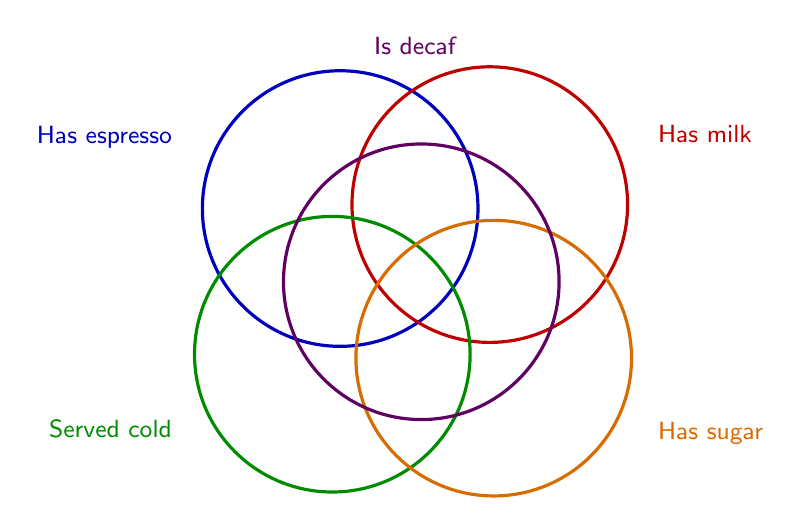
\begin{tikzpicture}[line width=1.15pt]
  % Five general-position circles.  Their boundaries are left unfilled so
  % every overlap remains legible.
  \draw[draw=blue!75!black]   (-0.95, 0.95) circle (1.75);
  \draw[draw=red!75!black]    ( 0.95, 1.00) circle (1.75);
  \draw[draw=green!55!black]  (-1.05,-0.90) circle (1.75);
  \draw[draw=orange!85!black] ( 1.00,-0.95) circle (1.75);
  \draw[draw=violet!75!black] ( 0.08, 0.02) circle (1.75);

  % Set names sit outside the circle boundaries; no connector marks are used.
  \node[blue!75!black,anchor=east,font=\sffamily\small]   at (-2.95, 1.85) {Has espresso};
  \node[red!75!black,anchor=west,font=\sffamily\small]    at ( 2.95, 1.90) {Has milk};
  \node[green!55!black,anchor=east,font=\sffamily\small]  at (-2.95,-1.85) {Served cold};
  \node[orange!85!black,anchor=west,font=\sffamily\small] at ( 2.95,-1.90) {Has sugar};
  \node[violet!75!black,font=\sffamily\small]             at (0, 3.02) {Is decaf};
\end{tikzpicture}
\end{document}
